\documentclass[04_projectProcess.tex]{subfiles}
\begin{document}
    \subsection{Ideas}
    \label{Ideas}

    \subsubsection{Color-changing Bracelet}
    \begin{flushleft}
        A color-changing bracelet was the first idea for the project. The bracelet would have 
        consisted of several parts. First, there are the main parts that include the microcontroller 
        and the battery and other sensors if needed. Threads are the second part. 
        Every thread can change its color if someone of your friends has such a thread as well, and 
        is close to you. Therefore, these bracelets can create a network, so they can communicate 
        with each other. The network strength can be used to identify if a friend is close. Then it 
        will change the color of the thread if the specific friend is close to the user. Also, groups 
        can be defined. Every group has its thread on the bracelet and if someone from the group 
        is next to you, the system changes the color of this specific thread (see Figure ~\ref{fig:braceltIdea}).
    \end{flushleft}

    \begin{figure}[H]
        \centering
        \begin{subfigure}{.45\textwidth}
            \centering
            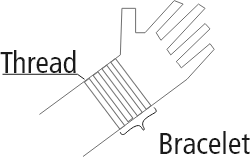
\includegraphics[scale=0.6]{images/projectideas/bracelt_1.png}
            \caption{Shows the bracelt concept.}
            \label{fig:braceltIdea}
            \vspace{6mm}
        \end{subfigure}
        \medskip
        \hspace{1mm}
        \begin{subfigure}{.45\textwidth}
            \centering
            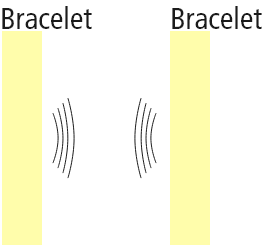
\includegraphics[scale=0.4]{images/projectideas/bracelt_2.png}
            \caption{Shows the bracelt concept.}
            \label{fig:braceltIdea}
            \vspace{6mm}
        \end{subfigure}
        \caption{Shows the color-changing bracelet idea and its functionality.}
        \label{fig:drillingProcess}
    \end{figure}

    \subsubsection{Music Controll Jacket}
    \begin{flushleft}
        Anyone knows the situation: You walk around in the city and it is very cold outside but you want 
        to change the song. Do you still do it? At this time, you don't want to grab the smartphone and 
        change the song you are listening to often because it is cold outside and you don't wanna freeze. \\
        So, another idea was to develop a jacket that can be used to change the song you are listening to 
        on a phone. Therefore, strips are placed on the left or right arm that can be used to play the 
        next or previous song in a playlist, make the song louder or quieter or stop the song playing 
        (see Figure ~\ref{fig:jacketIdea}).
    \end{flushleft}

    \begin{figure}[h!]
        \centering
        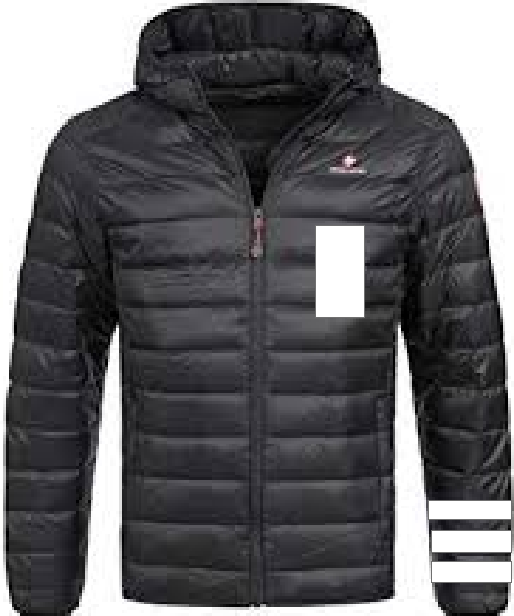
\includegraphics[scale=0.2]{images/projectideas/jacket.png}
        \caption{Shows the concept of a jacket with interaction areas.}
        \label{fig:jacketIdea}
    \end{figure}

    \subsubsection{Blossom Shaped Lamp}
    \label{BlossomShapedLamp}
    \begin{flushleft}
        A third and last idea is about lightning. The idea is to build a lamp of a blossom shape that 
        can be modified by the user. Every blossom leaf has a magnet inside, so it is possible to connect 
        each leaf. If some leaves are connected, LEDs that are in the middle of the flower blossom 
        change their color. Moreover, an analog slider can be used to change the brightness of the lamp 
        (see Figure ~\ref{fig:blossomLamp}).
    \end{flushleft}

    \begin{figure}[h!]
        \centering
        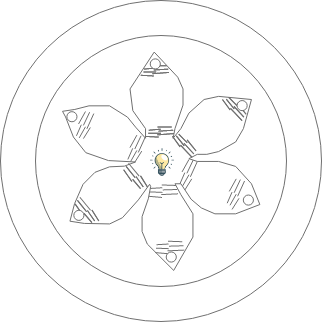
\includegraphics[scale=0.4]{images/projectideas/blossomLamp.png}
        \caption{Shows the concept of a blossom shaped lamp.}
        \label{fig:blossomLamp}
    \end{figure}
\end{document}